\chapter{INTRODUÇÃO}\label{chap:1}

Em 2017, o consumo de energia elétrica no mundo foi de~$21372\ TWh$~\cite{iea-consumo2017}.
É estimado que em 2030 esse consumo atinja cerca de~$27000\ TWh$ e em 2040 cerca de~$37000\ TWh$~\cite{iea2000-2040}.
Esse aumento é esperado devido à expectativa no aumento de veículos elétricos utilizados em todo o mundo.
Com o aumento no consumo de energia, serão necessários mais fontes de energia, causando ainda mais impactos na natureza.

A energia eólica contribui na redução do impacto ambiental causado pela produção de energia elétrica~\cite{cazzaro2019}.
A energia produzida pelas turbinas eólicas não gera poluentes como usinas que utilizam carvão, gás ou petróleo~\cite{saidur2011}.
As usinas nucleares entram na lista de energia limpa por não liberar substâncias na atmosfera~\cite{sadekin2019}, mas há controvérsias devido a criação de substâncias tóxicas e ao alto risco em caso de acidente~\cite{nirs2011, greenpeace2017}.
As hidrelétricas também são uma fonte limpa de energia, utilizando como combustível a água, porém utiliza barragens que bloqueiam o curso dos rios, alteram o fluxo de água e podem inundar áreas inteiras~\cite{koontz2015}.

Apesar de ser uma forma de produção limpa de energia, a fazenda eólica possui produção bastante variável e dependente do clima~\cite{fantidis2012}.
Já as hidrelétricas são bem menos sujeitas a variações, inclusive podendo armazenar água em um reservatório para suprir uma possível alta na demanda de energia~\cite{folk2018}.
A fonte de energia mais estável é a nuclear, produzindo em sua capacidade máxima cerca de~$92,6\%$ do tempo, enquanto hidrelétricas estão em capacidade máxima em~$42,8\%$ do tempo e as fazendas eólicas em~$37,4\%$~\cite{rone2018}.

O investimento para construção de uma fazenda eólica está entre as mais baratas se contruída em terra e entre as mais caras se construída no mar~\cite{eia2020}.
Gastos com a infraestrutura elétrica na construção de fazendas eólicas no mar variam entre~$15\%$ e~$30\%$ dos custos iniciais,~$12\%$ a~$26\%$ somente com os sistemas de coleta e transmissão de energia~\cite{gonzalez2014}.
Por isso, é bastante importante otimizar a forma com que os cabos são conectados até alguma subestação de energia.
Uma conexão direta entre cada turbina e a subestação é inviável.
Para reduzir os custos, cada turbina pode ser conectada em série por um a cabo a uma outra turbina, que pode estar conectada a outra, e assim sucessivamente até a subestação.
A Figura~\ref{fig:barrowfarm} mostra a topologia de uma fazenda real, Barrow, construída no mar da Irlanda.
Note que a conexão~$S01$--$C01$ é paralela à conexão~$S01$--$B01$, fazendo uma curva em torno da turbina~$B01$.

\begin{figure}[!htb]
  \centering
  \caption[Fazenda eólica Barrow]{
    Fazenda eólica Barrow no mar da Irlanda.
    Um círculo representa uma turbina, enquanto um quadrado representa uma subestação.
  }
  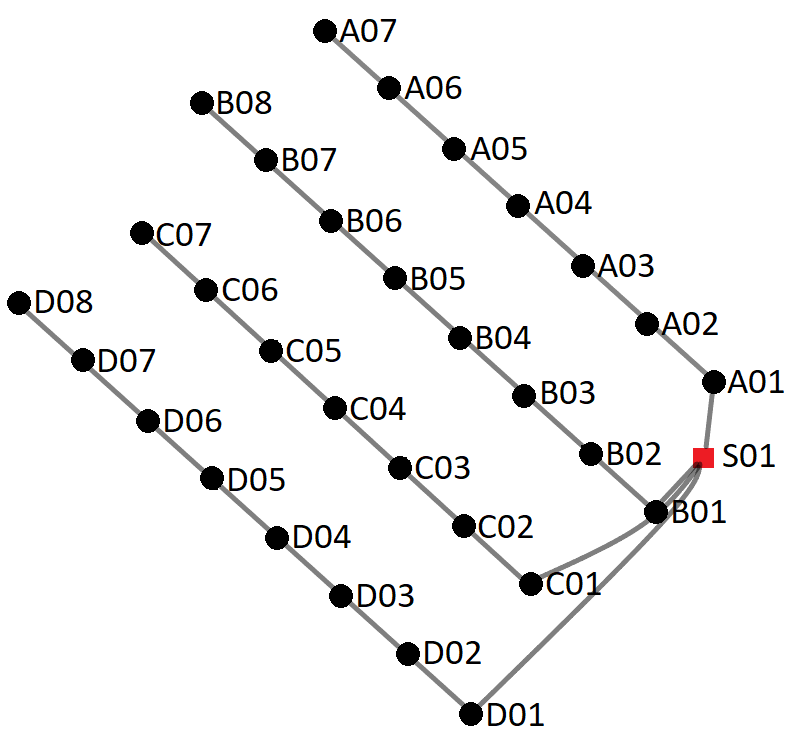
\includegraphics[scale=0.4]{estrutura/textuais/figuras/barrow-farm-connected.png}
  \caption*{Fonte: adaptado de~\citeonline{bauer2015}.}
  \label{fig:barrowfarm}
\end{figure}

Um requisito das empresas de energia é que não haja dois cabos cruzados, evitando uma possível remoção de um cabo para manutenção em outro~\cite{fischetti2017}.
Além disso, se dois cabos se cruzam, é necessário isolá-los, já que aquecem bastante devido a alta voltagem nos cabos~\cite{bauer2015}.

As fazendas eólicas podem ser cabeadas utilizando vários cabos ou apenas um cabo em comum para toda a fazenda.
A Figura~\ref{fig:barrow-optimal} mostra qual seria a topologia ótima utilizando os mesmos cabos do projeto original.

\begin{figure}[!htb]
  \centering
  \caption[Conexão ótima da fazenda Barrow]{
    Conexão ótima para a fazenda de Barrow utilizando os mesmos cabos utilizados inicialmente.
  }
  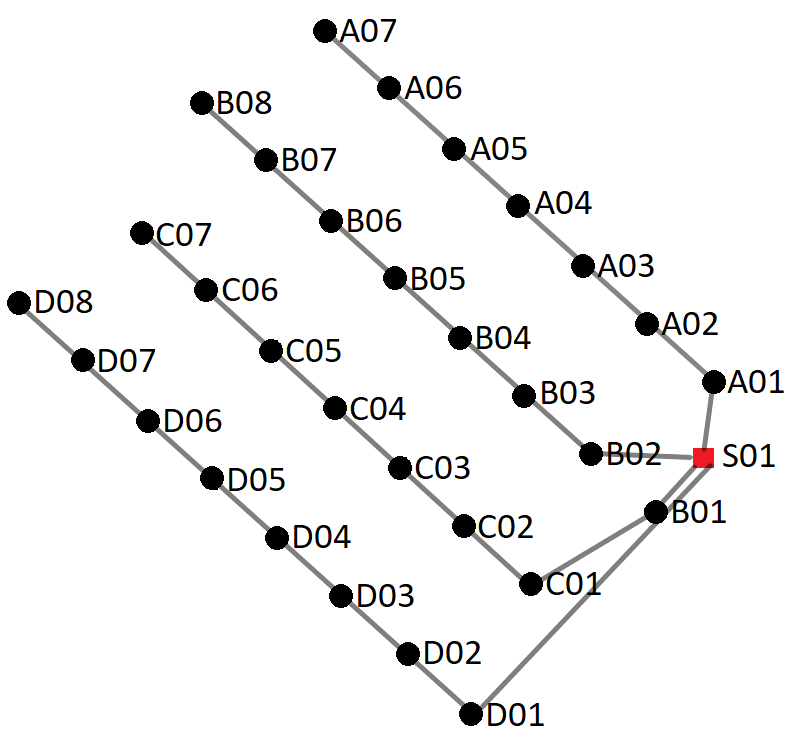
\includegraphics[scale=0.4]{estrutura/textuais/figuras/barrow-farm-optimal-same-cables.png}
  \caption*{Fonte: adaptado de~\citeonline{bauer2015}.}
  \label{fig:barrow-optimal}
\end{figure}

Existem diversos tipos de cabos disponíveis com custos diferentes.
Cada um possui suas vantagens, com resistência e capacidade elétrica diferentes.
Isso gera ainda mais opções de conexões, dando opção de escolher o cabo a ser utilizado em cada conexão.
Levando em consideração a resistência elétrica do cabo utilizado, o problema modela melhor a realidade e é possível planejar perdas de lucro a longo prazo.

Se adicionados pontos de Steiner, é possível modelar o desvio de um obstáculo, simulando uma curva em um cabo.
Esses pontos podem ser usados opcionalmente, não sendo obrigatório sua inclusão.
A Figura~\ref{fig:steinerexample} mostra um exemplo de um obstáculo.
Na figura, duas topologias são apresentadas, uma sem utilizar os pontos de Steiner e uma que os usa para simular um desvio.
Sem os pontos Steiner, a conexão~$(0, 19)$ exigiria um cabo que suporte~$14$ turbinas, enquanto a configuração que usa os pontos de Steiner deve suportar~$10$ turbinas no trecho menor~$(0$--$36)$.
Note que a alteração na topologia permite trocar outras conexões, o que pode melhorar o resultado.

\begin{figure}[!htb]
  \centering
  \caption[Exemplo de uso de pontos Steiner]{
    Exemplo de uso de pontos de Steiner para desviar de um obstáculo.
    A configuração à esquerda não utiliza pontos de Steiner, enquanto na configuração à direita utiliza para simular a curvatura do cabo e desviar do obstáculo.
  }
  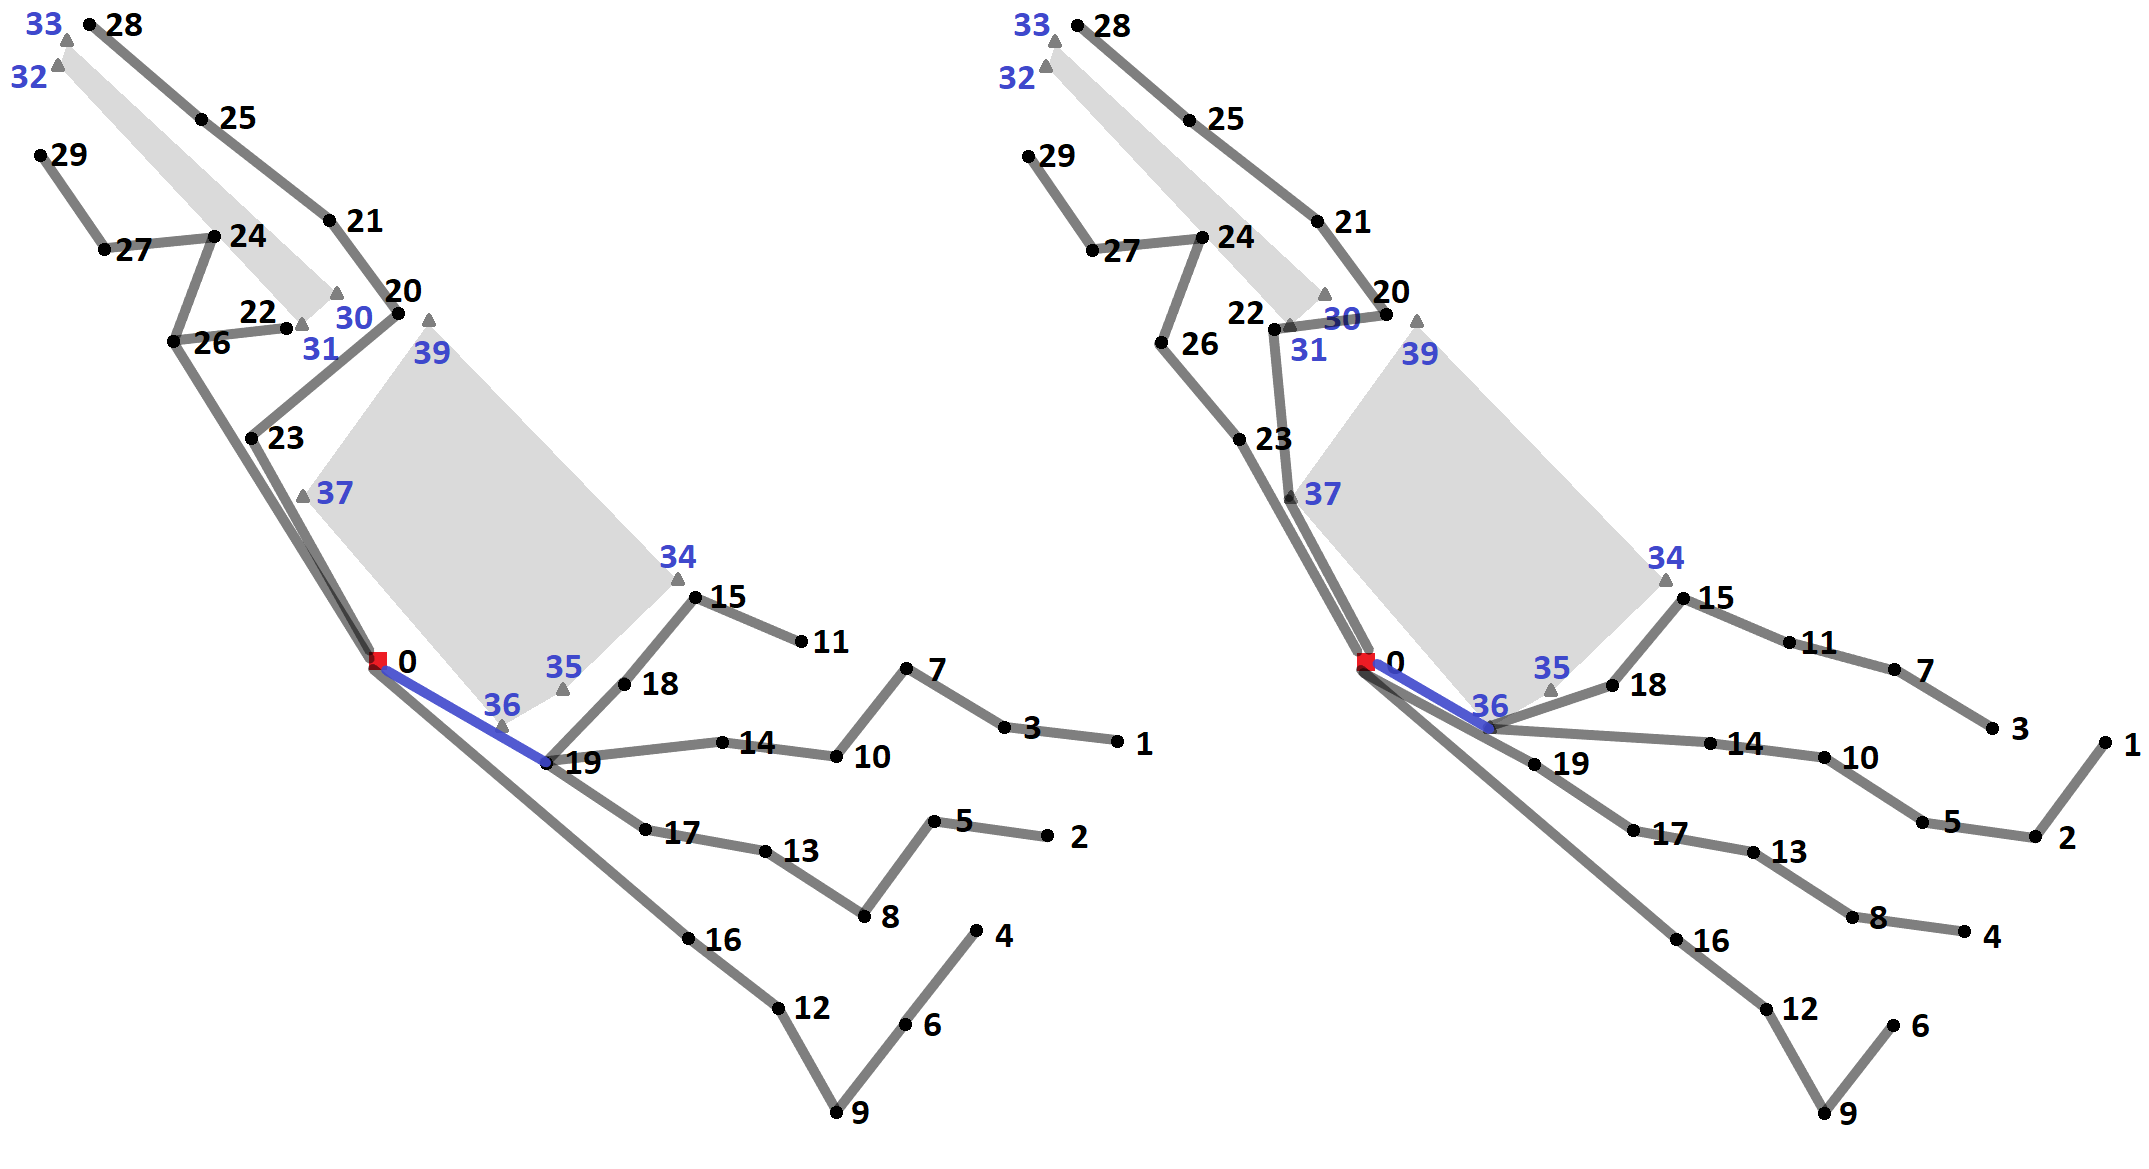
\includegraphics[scale=0.27]{estrutura/textuais/figuras/steiner-example-connected.png}
  \caption*{Fonte: adaptado de~\citeonline{fischetti2017}.}
  \label{fig:steinerexample}
\end{figure}

\section{Objetivos}

O objetivo deste trabalho de conclusão de curso é expor uma abordagem utilizando metaheurística para solução do problema de roteamento de cabos elétricos.
Será abordado apenas o problema de cabeamento, supondo que a definição da localização das turbinas, dos pontos de Steiner e da subestação já foram definidos.
Para reduzir o problema, a fazenda eólica será limitada a uma subestação, que é o que ocorre na maioria dos casos~\cite{cazzaro2019}.
A metaheurística deve: dado um conjunto de cabos, as posições de várias turbinas e de uma subestação, encontrar uma forma enonômica de colocar os cabos entre as turbinas de forma que a energia das turbinas flua para a subestação.

%\section{Organização textual}
